\section{Auswertung}
\label{sec:Auswertung}

\begin{figure}
  \centering
  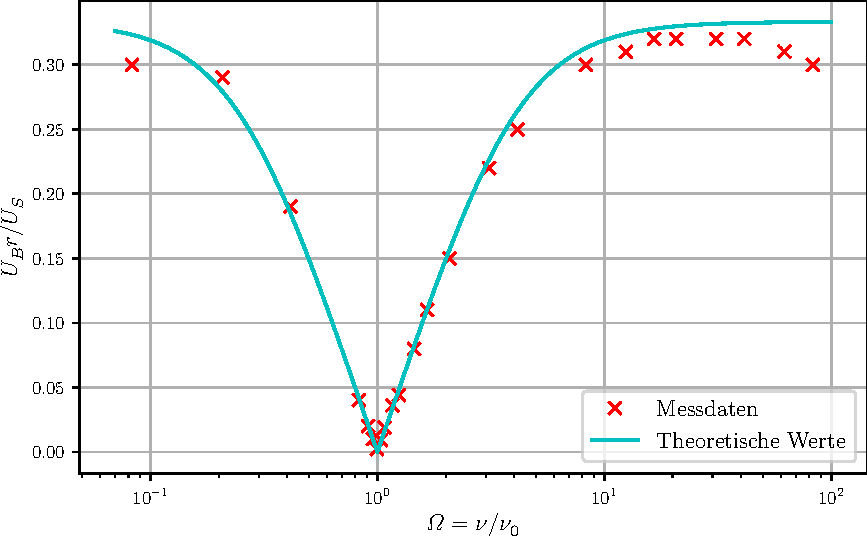
\includegraphics{plot.pdf}
  \caption{Plot.}
  \label{fig:plot}
\end{figure}

Nullmessung:
 Zählrate 828
 Messzeit 900 s


\begin{table}[H]
  \centering
  \caption{Messdaten zum $\gamma$-Zerfall mit Eisen als Absorber.}
  \label{tab:Zerfall2}
  \sisetup{table-format=2.2}
  \begin{tabular}{S[table-format=4.0] S[table-format=6.0] S[table-format=4.0] S S}
    \toprule
    \multicolumn{1}{p{2cm}}{ $ d/ \si{\milli\meter}$} &\multicolumn{1}{p{2cm}} {Messzeit $t / \si{\second}$} & \multicolumn{2}{p{2cm}}{$N$}& \multicolumn{2}{p{2cm}}{$N/t / \si{\per\second}$}\\
    \midrule
       0.0 &  60 &  6976 & 83.52 & 116.27 & 1.39 \\
       0.5 &  60 &  6738 & 82.09 & 112.30 & 1.37 \\
       1.0 &  60 &  6635 & 81.46 & 110.58 & 1.36 \\
       1.5 &  60 &  6374 & 79.84 & 106.23 & 1.33 \\
       2.0 &  60 &  6463 & 80.39 & 107.72 & 1.34 \\
       2.5 &  60 &  6261 & 79.13 & 104.35 & 1.32 \\
       3.0 &  60 &  5622 & 74.98 &  97.30 & 1.25 \\
       5.0 &  60 &  5410 & 73.55 &  90.17 & 1.23 \\
       6.0 &  60 &  5681 & 75.37 &  94.68 & 1.26 \\
       7.0 &  60 &  5318 & 72.92 &  88.63 & 1.22 \\
      10.0 &  60 &  4569 & 67.59 &  76.15 & 1.13 \\
      15.0 &  60 &  4101 & 64.04 &  68.35 & 1.07 \\
      20.0 &  60 &  2955 & 54.36 &  49.25 & 0.91 \\
      25.0 &  60 &  2428 & 49.27 &  40.47 & 0.82 \\
  \bottomrule
  \end{tabular}
\end{table}

Nt=  [116.26666667 112.3        110.58333333 106.23333333 107.71666667
 104.35        93.7         90.16666667  94.68333333  88.63333333
  76.15        68.35        49.25        40.46666667]
sigmaNt=  [1.392      1.36816667 1.35766667 1.33066667 1.33983333 1.31883333
 1.24966667 1.22583333 1.25616667 1.21533333 1.1265     1.06733333
 0.906      0.82116667]
Ntb=  [111.96666667  97.76666667  87.5         85.27777778  74.74444444
  66.25555556  58.74444444  41.78333333  39.42        35.75333333
  28.35        25.06111111]
sigmaNtb=  [1.366      1.2765     0.986      0.97344444 0.91133333 0.858
 0.80788889 0.59008333 0.51266667 0.4882     0.39688889 0.37311111]

\begin{table}[H]
  \centering
  \caption{Messdaten zum $\gamma$-Zerfall mit Blei als Absorber.}
  \label{tab:Zerfall2}
  \sisetup{table-format=2.2}
  \begin{tabular}{S[table-format=2.1] S[table-format=6.0] S[table-format=4.0]}
    \toprule
    \multicolumn{1}{p{2cm}}{ $ d/ \si{\milli\meter}$} &\multicolumn{1}{p{2cm}} {Messzeit $t / \si{\second}$} & \multicolumn{2}{p{2cm}}{$N$}& \multicolumn{2}{p{2cm}}{$N/t / \si{\per\second}$}\\    \midrule
       0.0 &  60 & 6718 & 81.96 & 111.97
       1.0 &  60 & 5866 & 76.59 & 
       2.0 &  90 & 7875 & 88.74 & 
       3.0 &  90 & 7675 & 87.61 & 
       4.0 &  90 & 6727 & 82.02 & 
       5.0 &  90 & 5963 & 77.22 & 
       6.0 &  90 & 5287 & 72.71 & 
      10.0 & 120 & 5014 & 70.81 & 
      11.0 & 150 & 5913 & 76.90 &
      12.0 & 150 & 5363 & 73.23 &
      14.0 & 180 & 5103 & 71.44 &
      15.0 & 180 & 4511 & 67.16 &
  \bottomrule
  \end{tabular}
\end{table}
Siehe \autoref{fig:plot}!
